\newpage
\section{Case Study \& Evaluation based on Taylor James paper}
\subsection{Weakness of the paper/Missing Elements}
According to the research paper by Taylor,IoT is an emerging technology that supports global infrastructure for exchange of information between ubiquitous computing devices without any interaction of humans. This paper describes the importance of practical and intelligence of Iot applications majorly in healthcare sector using a 5-Layered Architecture that represents its functionalities in an effective way.However there are few other factors that must be take care of such that IoHT devices can work efficiently\cite{5}.\\ \\
Few factors that require considerations are,
\begin{enumerate}
	\item Implementing Classical Middleware approach - Publish \& Subscribe method\\
	\item Introduction to Docker/Kubernetes\\
	\item Ensuring Privacy \& Security\\
\end{enumerate}
\subsubsection{Classical Middleware Approach-Publish\&Subscribe}
\hfill\\
\hfill\\
\emph{How can middleware approach of Publish \& Subscribe method help IoT Platform to meet their requirements?}\\ \\
IoHT comprises of various ubiquitous devices and technologies that offers real time data transmission of the surrounding and provide triggers based on the changes in the physical world.This methods lead to the approach of smart Healthcare,smart city,smart application and etc where billions of devices are connected over the internet for seemless interoperability.\\ \\
The classical sensor based devices deployed in IoT provide real time data but few devices have constraint where they can read the sensor data only once,which should be later distributed to several applications/services.To handle this challenge,a scalable cloud based messaging layer\cite{happ2017meeting},Publish and Subscribe model is used,that can match the data stream to the interested applications and distribute data accordingly.\\ \\
Pub/sub system mechanism ensures high performance processing and interoperability to allow devices to publish their presence(send data)to the node called as broker/router,which is responsible for traffic handling and distribution of data,and on the other side devices can subscribe to the broker for accessing the information based on their requirement.\\ \\
Pub/Sub is an asynchronous messaging service that decouples services that produce events from services that process events.It ensures message storage and real-time message delivery with high availability and consistent performance at high scale\cite{6}.\\ \\
Integrating publish/subscribe method in IoT platform is considered as the best approach for the interoperability and 
distributing various kinds of data over the network on different layers that acquires data from various other devices such as entities,devices,wireless sensors and etc.\\

\begin{figure}[H]
	\centering
	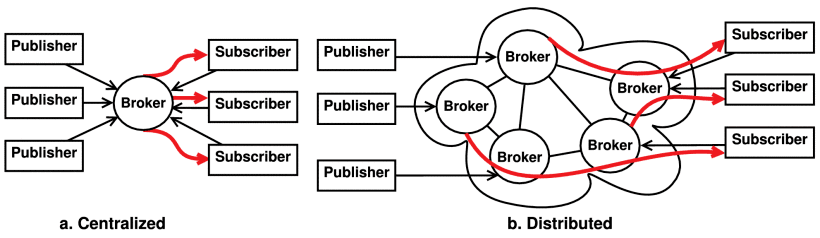
\includegraphics[width=\linewidth]{image/pub-sub.png}
	\caption{Publish-Subscribe System}
	\caption*{src:ElHassan et al\cite{4}}
\end{figure}

The usage of sensors and wireless technology for communication between the devices has lead to increased importance of wirless sensored networks in IoT.\\
Centralized pub/sub is more suitable for small network enterprise where as in case of large network consisting of many devices and heterogeneous data that uses topic-based filtering, Distributed pub/sub is very appropriate\cite{4}.\\ \\
Example:\\
PubSub thermostat: Controlling the fan based on the temperature change in IoT system,where the devices in this system publish temperature data on their pubsub registry feeds and individual device IDs. A server python application, which can run from any machine, consumes the data from Cloud based on Pub/Sub topic and events. The server then decides whether to turn on or off the individual devices fans via a Cloud IoT Core configuration update\cite{matthew}.
\subsubsection{Docker/Kubernetes}
\hfill\\
\hfill\\
\emph{Why is docker/kubernetes required in IoT Framework?}\\ \\ 
In recent years, cloud computing is an emerging field that deals with wide range of highly connected smart devices such as medical trackers,sensors,home appliances,and etc providing high computing power at low management effort.\\
As the developers deal with large number of devices,using containers can help them is many ways.\\ \\
Containers are lightweight when compared to virtual machines that uses lightweight kernel namescapes and runs on Build,Ship and Run Paradigm and virtualize the operating system and not the hardware which can enable applications run in isolation without affecting other applications making easy to move,modify and deploy with high security and scalability.\\ \\
The main idea of containers is to collect all the tools and libraries necessary to run a specific piece of software, and then isolating that software from the rest of the system. Because containers are not full-on virtual machines, they’re efficient, and Docker which is lightweight,standalone, is a leader in making containers easy to work with and share with others by ensuring better security and easy development\cite{8}.\\ \\

\begin{figure}[H]
	\centering
	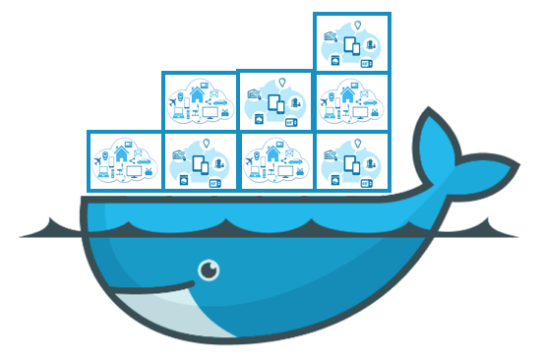
\includegraphics[width=10cm]{image/iot_containers.png}
	\caption{Docker Containers and IoT applications}
	\caption*{src:\cite{docker}}
\end{figure}

Docker,"the worlds leading software container platform and a tool that helps to solve common problems like installing,removing,upgrading,
distributing,trusting and managing software and provides a modern solution to tackle common software problems"\cite{7}.\\ \\
It is easy to maintained and deployed upon the virtulization machines.In IoT Framework,Applications that run different services on many devices make it reasonable to utilize a technology providing easy deployment and high portability within a distributed system environment\cite{7}.\\ \\
By using docker,the main challenges in IoT devices can be solved by enabling minimal hardware resources,highly scalable,distribution across the network,
limited network access and heterogeneous device environments.\\ \\
\begin{figure}[H]
	\centering
	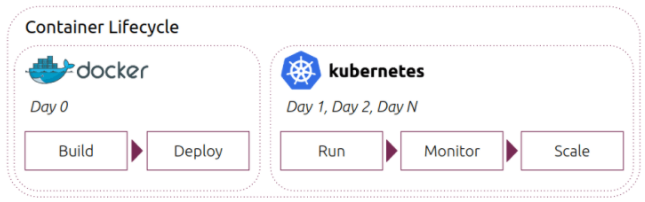
\includegraphics[width=\linewidth]{image/dockub.png}
	\caption{Docker and Kubernetes}
	\caption*{src:\cite{kub}}
\end{figure}
To automate these functionalities on a large scale,Kubernetes,an open source platform is what is required which gives system admin more control on the containers for deploying,scaling,managing and automates the processes in containerized application.Kubernetes benefits IoT as developers need not worry about the hardware or opeating system specifications and the property of self-healing makes the system more robust and reliable.With this ability,healthcare organizations in IoT platform implement both docker and kubernetes technology to reduce cost and time,provide high security,self-healing,quick deployment of application and highly scalable.\\ \\


\subsubsection{Privacy \& Security}
\hfill\\
\hfill\\
\emph{Why privacy and security is important in IoT?}\\ \\
Privacy and security is one of the key challenges faced by IoT in order to ensure secure and encrypted communication among billions of devices collecting data through wireless network.Most of the security issues faced during communication are Malicious code injection,sniffing attack,Denial of service,proxy attack and etc.There are few other factors such as proxy attack and man-in-the-middle attack that occurs irrespective of the connectivity being encrypted or not\cite{sec}.Hence it is necessary to ensure a secure and reliable communication protocols at all stack layers.\\ \\

\begin{figure}[H]
	\centering
	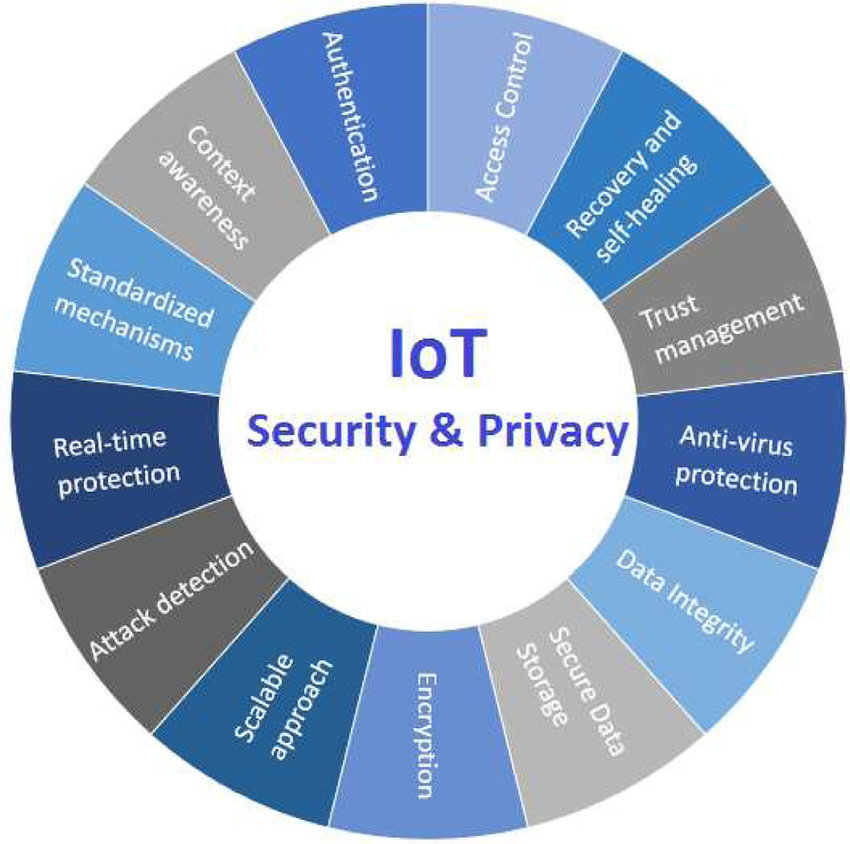
\includegraphics[width=8cm]{image/security.png}
	\caption{IoT security and privacy concerns}
	\caption*{src:\cite{sec}}
\end{figure}

The new Fog computing framework allows storing and processing the data at edge/cloud-to-endpoint continuum by overcoming the limitation of IoT devices.In general distributed systems are more vulnerable to attacks when compared to centralized systems.\\
Cloud usually operates in heavily protected facilities and managed by cloud operators where as Fog needs to function in more vulnerable environments by meeting customers requirements.As fog has resources smaller when compared to cloud it may not protect itself because of limilited resources.\\
Hence there are many privacy and security issues in Fog architecture that has to be addressed such as authentication,secure communication,confidentiality and authorization.\\
Inspite of cloud-platform providing advanced cryptosystem to enhance security,it cannot be implemented on resource-constraint devices in Fog as many devices are located in various locations and the chances of malicious activities are high\cite{9}.\\
 %https://www.hindawi.com/journals/wcmc/2018/9373961/
In order to deal with such problems,WebRTC(Web Real time communication) an open-source web-based application technology,is made use of which has the ability to deal with security issues in real-time communication by enabling and encouraging important security concepts at stack level.OpenTrust Protocol(OTrP) is used by applications to install,update,delete and manage security configurations.IPSec(Internet Protocol Security) is used in network layer which provides a end to end secure and transparent connection-oriented channel is used which is easier to run than TLS(Transport Layer security).Few applications rely on SSl(Secure socket layer) and DTLS(Datagram Transport Layer security) for secure data transmission.To deal with the Man-in-middle attack, media paths should be regularly monitored and should be coupled with encrypted signals for no spectical threat\cite{sec}.\\ \\
As the system grows large with enoromous data,it is always benificial to adapt lightweight protocols and encryption algorithms for better security in IoT environments and each object should check other's privacy policy for compatability before sharing data,as each system has its own privacy policies.Security and privacy is no longer an option but a must requirement in all fields.
